
\chapter{METHODOLOGY/MODEL EQUATION}


\section{{\bf{Conceptual Framework - Truss}}}
    Truss is a structure consisting of organized objects in a shape of connecting triangles in such a way that it behaves as a single unit object. In order to enable the distribution of weight and grasp up the the fluctuating tension and compression without bending and shearing, it is made up of a web of triangles which is most stable form of geometry. In general, truss is used since it has a long life span and has least weight to the possible which in turn supports large loads and reduces deflections.\\
    
    \begin{figure}
    	\centering
    	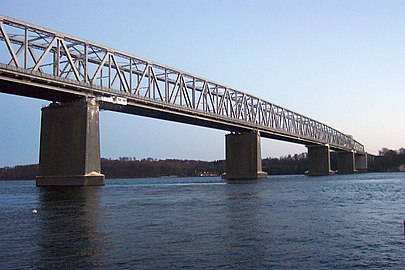
\includegraphics[width=0.4\linewidth , height=0.3\linewidth]{3}
    	\caption{Truss in bridge}
    \end{figure}
%  
    \begin{figure}
    	\centering
    	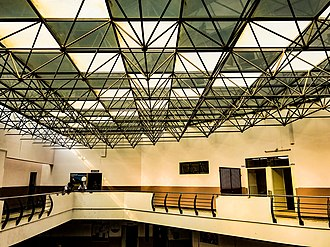
\includegraphics[width=0.4\linewidth , height=0.3\linewidth]{2}
    	\caption{Truss in roofing}
    \end{figure}    
    \begin{figure}
    	\centering
    	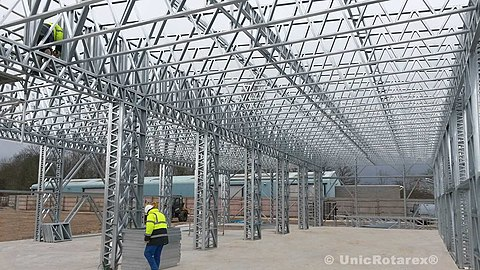
\includegraphics[width=0.4\linewidth , height=0.3\linewidth]{5}
    	\caption{Three Dimensional Truss}
    \end{figure}
    

Commonly used in bridges, roofs and high rise buildings, it gives high value for mega constructions like the Eiffel Tower, construction of a stadium and all. We can think of truss as a beam where the web consists of series of separate members instead of a continuous plate. In engineering perspective, a truss is a structure that comprises of one or more triangular units constructed in a linear pattern such that its ends are connected to joints which is called as external nodes. The external forces and reaction to the forces are considered to act only at the nodes and the results in forces in the members are either tensile or compressive forces. In truss, the lower horizontal structure and the upper horizontal structure carry tension and compression. The diagonal and vertical structure form the truss web and it carries shear stress. Technically, they are also in tension and compression where the exact arrangement of forces depends on the type of truss and on the direction of bending. The structures serves in order to stabilize each other in order to prevent buckling. The structures that are under compression are to be designed to be safe against buckling. After knowing the force on each member, we determine the cross sectional area of the individual truss members. The weight of truss structure depends directly on its cross section area. The effect of weight of individual structures in a large truss is generally insignificant compared to the force exerted by external loads.\\

Later, after determining the minimum area of cross section of individual structures, it is dealt with bolted joints that involves shear stress of the bolt and connections used in the joints. The joints of truss can be designed as rigid, semi-rigid, or hinged.\\

Equation of truss: \\

The strain-displacement relationship is: \\
\begin{eqnarray}
	\epsilon = \frac{du}{dx}\\
	\sigma = E\epsilon
\end{eqnarray}

From the law of equilibrium, we get,
\begin{eqnarray}
	A\sigma_x = T = constant
\end{eqnarray}

Combining, the equations, we get:
\begin{eqnarray}
	AE\frac{du}{dx} = T = constant
\end{eqnarray}

Differentiating with respect to x, we get,
\begin{eqnarray}
	\frac{d}{dx}(AE\frac{du}{dx}) = 0
\end{eqnarray}
is the equation of truss.

\pagebreak
\section{\bf{Mathematical Model and solution methods}}
%part assigned to samrajya

Consider\\
\begin{eqnarray}
	-\frac{d}{dx} \left[a(x)\frac{du}{dx} \right] = f(x)  \quad\quad  \text{for} \quad\quad  0<x<L.
\end{eqnarray}
for $u(x)$ subject to the boundary conditions\\
\begin{eqnarray}
	u(0)= u_0 \\
	a(x)\frac{du}{dx}\biggr|_{x=L} = Q_L	
\end{eqnarray}
where $a(x)$ and $f(x)$ are known functions and 
$u_0$ and $Q_L$ are known values.
In case of bar (which is a axially loaded structure) , the variables denote these quantities:
\begin{eqnarray*}
	u = \text{displacement}\\
	a(x)= \text{EA (stiffness)}\\
	f = \text{distributed axial force}\\
	Q_L= \text{axial load}
\end{eqnarray*}
Our goal is to determine the function $u(x)$. Since analytic or exact solution is not feasible, we want an approximation of u(x) in the form
\begin{eqnarray}\label{approxfunc}\label{approxsoln}
	u(x)\approx u_N(x) = \sum\limits_{j=1}^N c_j\phi_{j} + (x) +\phi_{0}(x)
\end{eqnarray}

%%page 2 of copy

 Substituting  $U_N$(x) in our Differential Equation, 
 \begin{eqnarray}
 	-\frac{d}{dx} \left[a(x)\frac{dU_N}{dx} \right] = f(x)  \quad\quad  \text{for} \quad\quad  0<x<L.
 \end{eqnarray}

If this equally holds for all $x \in [0,L] $ the solution is exact. Since, it is only an approximation , we define residual function $R(x,c_1, c_2, c_3,...,c_N)$ to check the how close the approximation is to our original problem.
\begin{eqnarray}
	R = -\frac{d}{dx} \left[a(x)\frac{dU_N}{dx} \right] - f(x)
\end{eqnarray} 

We have R $\neq$0 $ \forall x  \in [0, L]$  as $U_N$ is only a approximation to solution.
\pagebreak

Now we have various ways to minimize R in some senses over the domain to make this approximation close to the actual solution. At this point all we want to do is to get N conditions to impose on the R in such a way that we obtain N linear equations in the unknown coefficients $c_1, c_2, c_3,...,c_N$.
This is allow us to determine the coefficients in our approximation as in equation \ref{approxfunc}
\begin{enumerate}
	\item Collocation Method\\
	It forces that R is zero at selected N points of the domain.\\
	i.e; 
	\begin{eqnarray}
		R(x,c_1, c_2, c_3,...,c_N) = 0  \quad\quad\quad \forall x=x_i, i = 1,2,...,N
	\end{eqnarray}

	\item Least Square Method
		\begin{eqnarray}
			\frac{\partial}{\partial c_j} \int_{0}^{L} R^2 dx = 0 \quad\quad\quad \forall i = 1,2,...,N
		\end{eqnarray}
	
	\item Weighted Residual Method
		we desire that 
			\begin{eqnarray}\label{weightedintegralgen}
				\int_{0}^{L} w_i(x) R dx = 0 \quad\quad\quad \forall i = 1,2,...,N
			\end{eqnarray}
		where $w_i(x)$ are N linearly independent functions called weight functions.
		
		Choice of weight functions is totally arbitrary but there are some standard ways to choose the weight function which have been assigned special names. If we let $w_i = \phi_i$ , then the method is known as \textbf{galerkin's method.}
\end{enumerate}

%page 4
	Now we convert our differential equation and boundary condition to weak form to make it easier to choose approximation functions.
\begin{itemize}
	\item Step 1 :
	We write the weighted integral statement from eqn \ref{weightedintegralgen}, i.e;
	\begin{eqnarray}\label{weightedint}\label{weightedintform}
		\int_{0}^{L}  w \left[ -\frac{d}{dx} \left( a(x)\frac{du}{dx} \right) - f \right] dx = 0
	\end{eqnarray}

	It is equivalent to differential equations and does not include any boundary conditions and moreover the variable $u$ must be differentiable to as many order as is required by the differential equation.
	\item Step 2:\\
	to weaken differentiability conditions for $u(x)$, let us rewrite our eqn \ref{weightedint} as,
	\begin{eqnarray}
		\int_{0}^{L}  \left( w \left[ -\frac{d}{dx} \left( a(x)\frac{du}{dx} \right) \right] - wf \right)  dx = 0
	\end{eqnarray}
	Integrating by parts, we get,
	\begin{eqnarray}\label{weakform1}
		\int_{0}^{L} \left[ a \frac{dw}{dx} \frac{du}{dx} - wf \right] dx  - \left[ wa \frac{du}{dx}\right]_0^L = 0
	\end{eqnarray}

%%page 5 of copy

	we have used the fact that 
	\begin{eqnarray}
		\int_{a}^{b} \left( w \frac{dv}{dx} \right)dx  =  -\int_{a}^{b} v dw + \left[wv\right]_0^L = 0
	\end{eqnarray}

by considering,
	\begin{eqnarray}
		v = -a\frac{du}{dx}
	\end{eqnarray}

we can see that now we require that w be differentiable at least once but this also made that u needs to be differentiable only once even though the equation is of second order.\\
    \item Step 3:\\
    Now, we take care of the boundary conditions which are of two types
\begin{itemize}
	\item Natural Boundary  condition
	\item Essential Boundary Condition 
\end{itemize}

Before defining these conditions we define primary and secondary variables.

\begin{df}[Primary Variable]
	The coefficients of the weight function (and its derivatives) in the boundary expressions is called primary variable.
\end{df}

\begin{df}[Secondary Variable]
	The dependent variable of the problem($u$), expressed in the same form as the weight function ($w$) appearing in the boundary tern is called primary variable.
\end{df}

In our case , $u(x)$ is the primary variable and  $ a \frac{du}{dx}$ is secondary variable.

If secondary variable(SV) is specified in the boundary, then such conditions are called \textbf{natural boundary conditions} (NBC).
If primary variable(PV) is specified in the boundary, then such conditions are called \textbf{essential boundary conditions} (NBC).

let us now define secondary variable as Q.
\begin{eqnarray}
	Q = a\frac{du}{dx} n_x
\end{eqnarray}

where $n_x$ is the cosine of the cosine of the angle between the positive x-axis and the normal to the boundary.

For 1D problems,

\begin{eqnarray}
	n_x = -1 \quad\quad\quad \text{at left}\\
	n_x = 1 \quad\quad\quad \text{at right}
\end{eqnarray}

%Page 7 from copy
	To utilize these new facts , we use the equation \ref{weakform1}
	\begin{eqnarray}
	\int_{0}^{L} \left[ a \frac{dw}{dx} \frac{du}{dx} - wf \right] dx  - \left[ wa \frac{du}{dx}\right]_0^L = 0
    \end{eqnarray}

	\begin{eqnarray}
	\implies	\int_{0}^{L} \left[ a \frac{dw}{dx} \frac{du}{dx} - wf \right] dx  + wa\frac{du}{dx}\biggr|_{x=L} - wa\frac{du}{dx}\biggr|_{x=0} = 0
	\end{eqnarray}
	since $n_x = -1 \quad \text{at} \quad x = 0 $ and $n_x = 1 \quad \text{at} \quad x = L$
	\begin{eqnarray}
	\implies	\int_{0}^{L} \left[ a \frac{dw}{dx} \frac{du}{dx} - wf \right] dx  - n_xwa\frac{du}{dx}\biggr|_{x=L} - n_xwa\frac{du}{dx}\biggr|_{x=0} = 0
	\end{eqnarray}
	\begin{eqnarray}\label{expandedweak}
	\implies \int_{0}^{L} \left[ a \frac{dw}{dx} \frac{du}{dx} - wf \right] dx  -(wQ)_0  -(wQ)_L = 0
	\end{eqnarray}
	Weight functions can be interpreted as virtual change of the primary variable ($ w \approx \delta u $)
	thus we require that weight functions vanishes at boundaries where essential boundary conditions are specified as at such points the value of u is known exactly.
	\begin{eqnarray}
		u(0) = u_0 \implies w(0) = 0
	\end{eqnarray}
Thus, we get
	\begin{eqnarray}
		\int_{0}^{L} \left[ a \frac{dw}{dx} \frac{du}{dx} - wf \right] dx   -w(L)Q_L = 0
	\end{eqnarray}

	
\end{itemize}
%part after assigning to samrajya
Let us define two functionals $B$ and $l$ as,
\begin{eqnarray}
	B(w,u) = \int_{0}^{L} a \frac{dw}{dx} \frac{du}{dx} dx \\
	l(w) = \int_{0}^{L} wf dx + w(L) Q_L
\end{eqnarray}

Hence, our weak form can be written as

\begin{eqnarray}
	0 = B(w,u) - l(w)
\end{eqnarray}
or ,
\begin{eqnarray}\label{variational}
	B(w,u) = l(w)
\end{eqnarray}

This is the variational form of the problem that is associated with our ODE and its boundary conditions.

When the differential equation is linear and of even order, the resulting weak form will have symmetric bi-linear form in u and w.

We will now use ritz-galerkin , we will obtain the linear equations to obtain the coefficients which we used to define the \ref{approxfunc} by using the above vairational form.

for Ritz method , we substitute $w_i = \phi_i$ hence eqn \ref{variational} becomes

\begin{eqnarray}
	B \left(\phi_i, \sum_{1}^{N} c_j \phi_j + \phi_0 \right) = l(\phi_i)  \quad\quad\quad i = 1,2,...,N
\end{eqnarray}

Since $B(\cdot , \cdot ) $ is bilinear , it is linear in u. hence,

\begin{eqnarray} \label{linearBl}
	\sum_{1}^{N} B \left(\phi_i, \phi_j \right)  c_j  = l(\phi_i) -  B \left(\phi_i, \phi_0 \right)  \quad\quad\quad i = 1,2,...,N
\end{eqnarray}

Let , 
\begin{eqnarray}\label{gencoeff}
	K_{ij} = B(\phi_i , \phi_j) \\
	F_i = l(\phi_i) - B(\phi_i , \phi_0)
\end{eqnarray}

Then eqn \ref{linearBl} can be written in matrix form as
\begin{eqnarray}
	\boldmath{K} c = \boldmath{F}
\end{eqnarray}

Since $K$ and $f$ are completely determined ,we can easily compute the coefficients.

The last hurdle towards writing down the approximate solution exactly is choosing the approximate functions $\phi_i$ appropriately.

Firstly we must make sure that these functions satisfy the essential boundary conditions. Since, the natural boundary conditions are already included in the weak form, this is the last step to properly apply all the given boundary conditions.

We can demand that
\begin{eqnarray}
	\phi_0(x_0) = u_0\\
	\sum_{1}^{N} c_j \phi_j(x_0) = 0
\end{eqnarray} 

We will obtain 
\begin{eqnarray}
	U_N(x_0) = u_0
\end{eqnarray}
and hence the essential boundary conditions are satisfied.
 
It is obvious that these functions must be as differentiable and integrable as the weak form demands. In addition, we want these to be complete set of \textbf{linearly independent functions}.

Thus variational method provides us with a powerful method to solve equations. provided we can compute the integrals in case of complex geometry as the discussion encompasses the entire domain of the problem at once. Since, this is not always possible for complex geometry or material property, we discritize our domain into line elements. A typical element between points A and B with coordinates $x_a$ and $x_b$ respectively, is denoted $\Omega_e$. The length of element is $h_e = x_b - x_a$. 

Now we follow the above steps to obtain the approximate solution ($u_h^e$) over this element.
The approximate solution is assumed to be opf the form 
\begin{eqnarray}
	u_h^e = \sum_{j = 0 }^{N} u_j^e \psi_j^e(x)
\end{eqnarray} 
Here $ u_j^e$ and $\psi_j^e(x)$ are the coefficients and the approximation functions respectively. 

Writing eqn \ref{weightedintform} for our element's domain,
\begin{eqnarray}
			\int_{x_a}^{x_b}  w \left[ -\frac{d}{dx} \left( a(x)\frac{du}{dx} \right) - f \right] dx = 0
\end{eqnarray}

Similarly, the final weak form can be written from eqn \ref{expandedweak} as 

\begin{eqnarray}
	 \int_{x_a}^{x_b} \left[ a \frac{dw}{dx} \frac{du}{dx} - wf \right] dx  -(wQ)_a  -(wQ)_b = 0
\end{eqnarray}

let us also write the corresponding variational form,
\begin{eqnarray}\label{variational}
	B^e(w,u) = l^e(w)
\end{eqnarray}
where,
\begin{eqnarray}
	B^e(w,u) = \int_{x_a}^{x_b} a \frac{dw}{dx} \frac{du}{dx} dx \\
	l^e(w) = \int_{x_a}^{x_b} wf dx + w(x_a) Q_a + w(x_b) Q_b
\end{eqnarray}

% Choosing approximate functions

Let us now choose the approximate solutions that satisfy the two conditions for primary variables as other conditions are already included in the weak form. 
i.e,

\begin{eqnarray}
	u_h^{e} (x_a) = u_1^{e} \\
	u_h^{e} (x_b) = u_2^{e}  
\end{eqnarray}
let,
\begin{eqnarray}
	u_h^{e} (x) = c_1 + c_2 x
\end{eqnarray}

Then by the conditions,

\begin{eqnarray}
	u_h^{e} (x_a) = c_1 + c_2 x_a = u_1^{e}\\
	u_h^{e} (x_b) = c_1 + c_2 x_b = u_2^{e}
\end{eqnarray}

writing in matrix form, we obtain
\begin{eqnarray}
\begin{bmatrix}
	u_1^{e}\\
	u_2^{e}
\end{bmatrix}
=
\begin{bmatrix}
	1 & x_a\\
	1 & x_b
\end{bmatrix}
\begin{bmatrix}
	c_1^{e}\\
	c_2^{e}
\end{bmatrix}
\end{eqnarray}

We can rewrite the equations as 
\begin{eqnarray}
	\begin{bmatrix}
		c_1^{e}\\
		c_2^{e}
	\end{bmatrix}
	= \frac{1}{x_b - x_a}
	\begin{bmatrix}
		x_b & -x_a\\
		-1 & 1
	\end{bmatrix}
	\begin{bmatrix}
		u_1^{e}\\
		u_2^{e}
	\end{bmatrix}
\end{eqnarray}

Hence we get,

\begin{eqnarray}
	c_1^{e} = \frac{1}{h_e} (x_bu_1^e - x_bu_2^e)
\end{eqnarray}
\begin{eqnarray}
	c_2^{e} = \frac{1}{h_e} (-u_1^e + u_2^e)
\end{eqnarray}

If we let,
\begin{eqnarray*}
	\alpha_1^e = x_b\\
	\alpha_2^e = - x_a\\
	\beta_1^e = -1 \\
	\beta_2^e = 1	
\end{eqnarray*}

\begin{eqnarray}
	c_1^{e} = \frac{1}{h_e} (\alpha_1^e u_1^e + \alpha_2^e u_2^e)
\end{eqnarray}
\begin{eqnarray}
	c_2^{e} = \frac{1}{h_e} (\beta_1^eu_1^e + \beta_2^e u_2^e)
\end{eqnarray}

Hence,
\begin{eqnarray*}
	U_h^e(x) =  \frac{1}{h_e} [\alpha_1^e u_1^e + \alpha_2^e u_2^e + (\beta_1^eu_1^e + \beta_2^e u_2^e)x]
\end{eqnarray*}
\begin{eqnarray*}
	U_h^e(x) =  \frac{1}{h_e} [\alpha_1^e + \beta_1^e x] u_1^e + \frac{1}{h_e} [\alpha_2^e + \beta_2^e x] u_2^e
\end{eqnarray*}
\begin{eqnarray}
U_h^e(x) = \sum_{j=1}^{2} \frac{1}{h_e} [\alpha_j^e + \beta_j^e x] u_j^e 
\end{eqnarray}

\begin{eqnarray}
	U_h^e(x) = \sum_{j=1}^{2} \psi_j^e(x) u_j^e 
\end{eqnarray}

where $\psi_j^e(x)$ are known as interpolation functions. It can be seen that $\psi_j^e(x)$ are simply Lagrange interpolation functions and can be written quite succinctly as,
    \begin{figure}[h!]
	\centering
	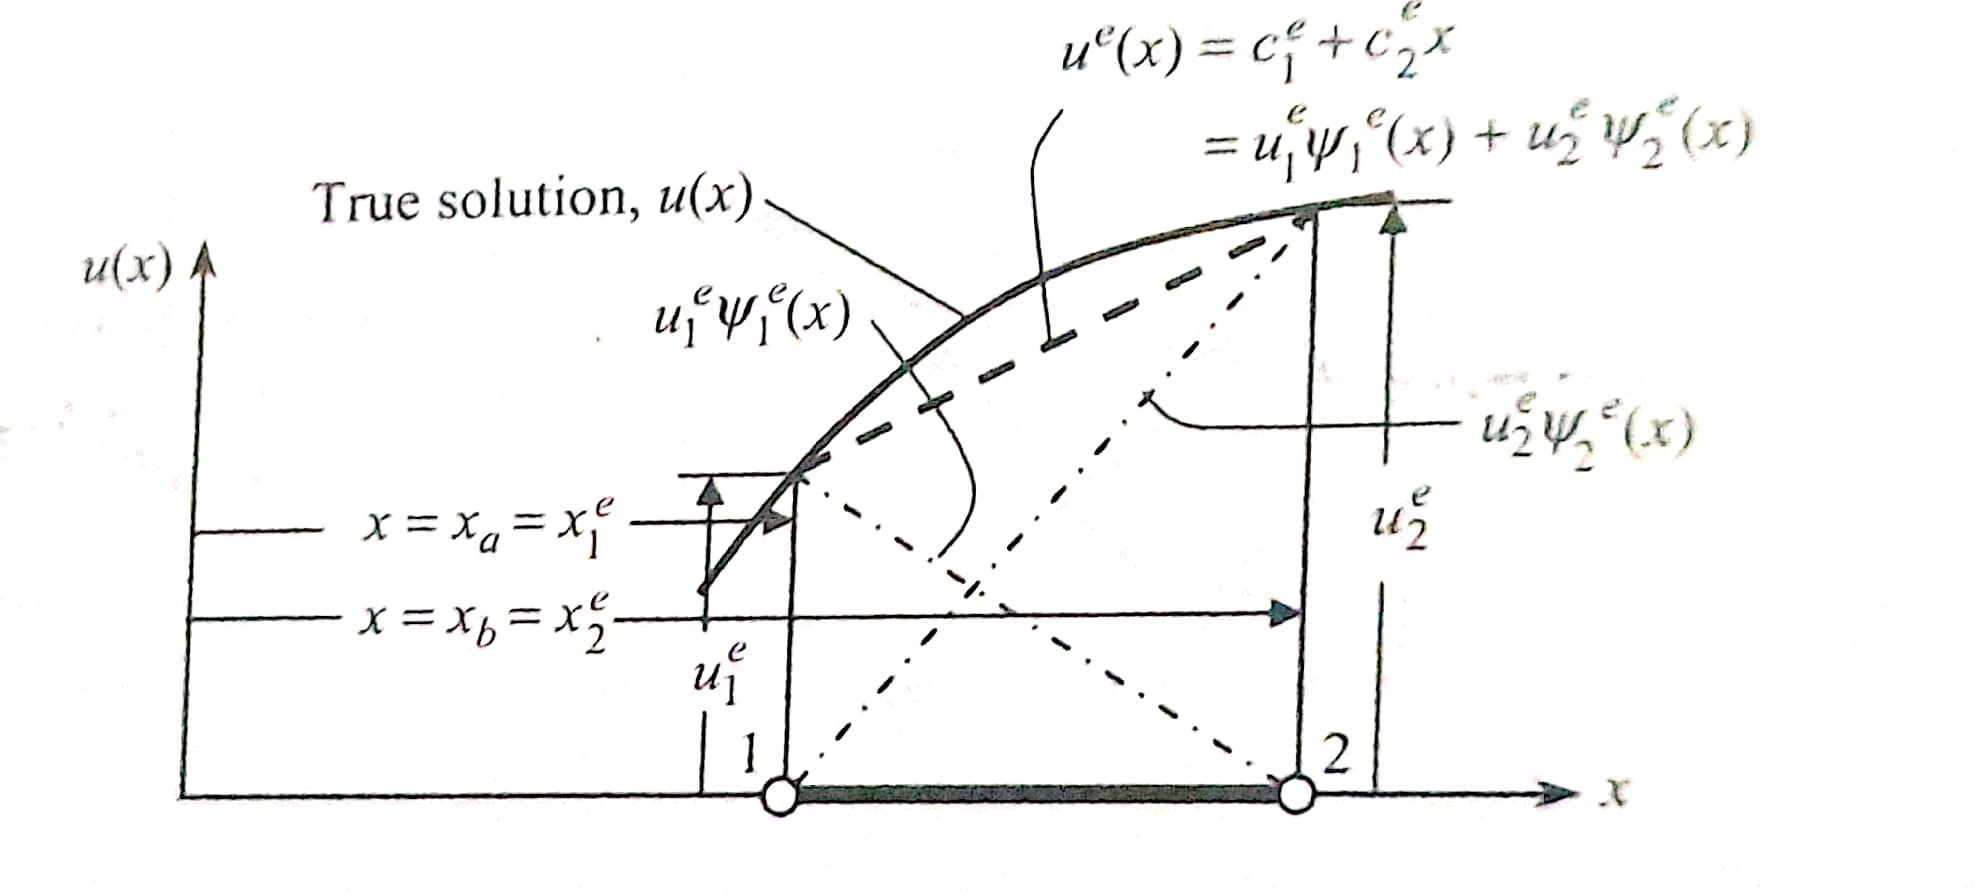
\includegraphics[width=0.9\linewidth , height=0.4\linewidth]{T6}
	\caption{Linear Lagrange Interpolation Functions}
\end{figure}
\begin{eqnarray}\label{locallagrange}
	\psi_1^e(\bar{x}) = 1 - \frac{\bar{x}}{h_e} , \quad\quad \psi_2^e(\bar{x}) = \frac{\bar{x}}{h_e}
\end{eqnarray}
    \begin{figure}[h!]
	\centering
	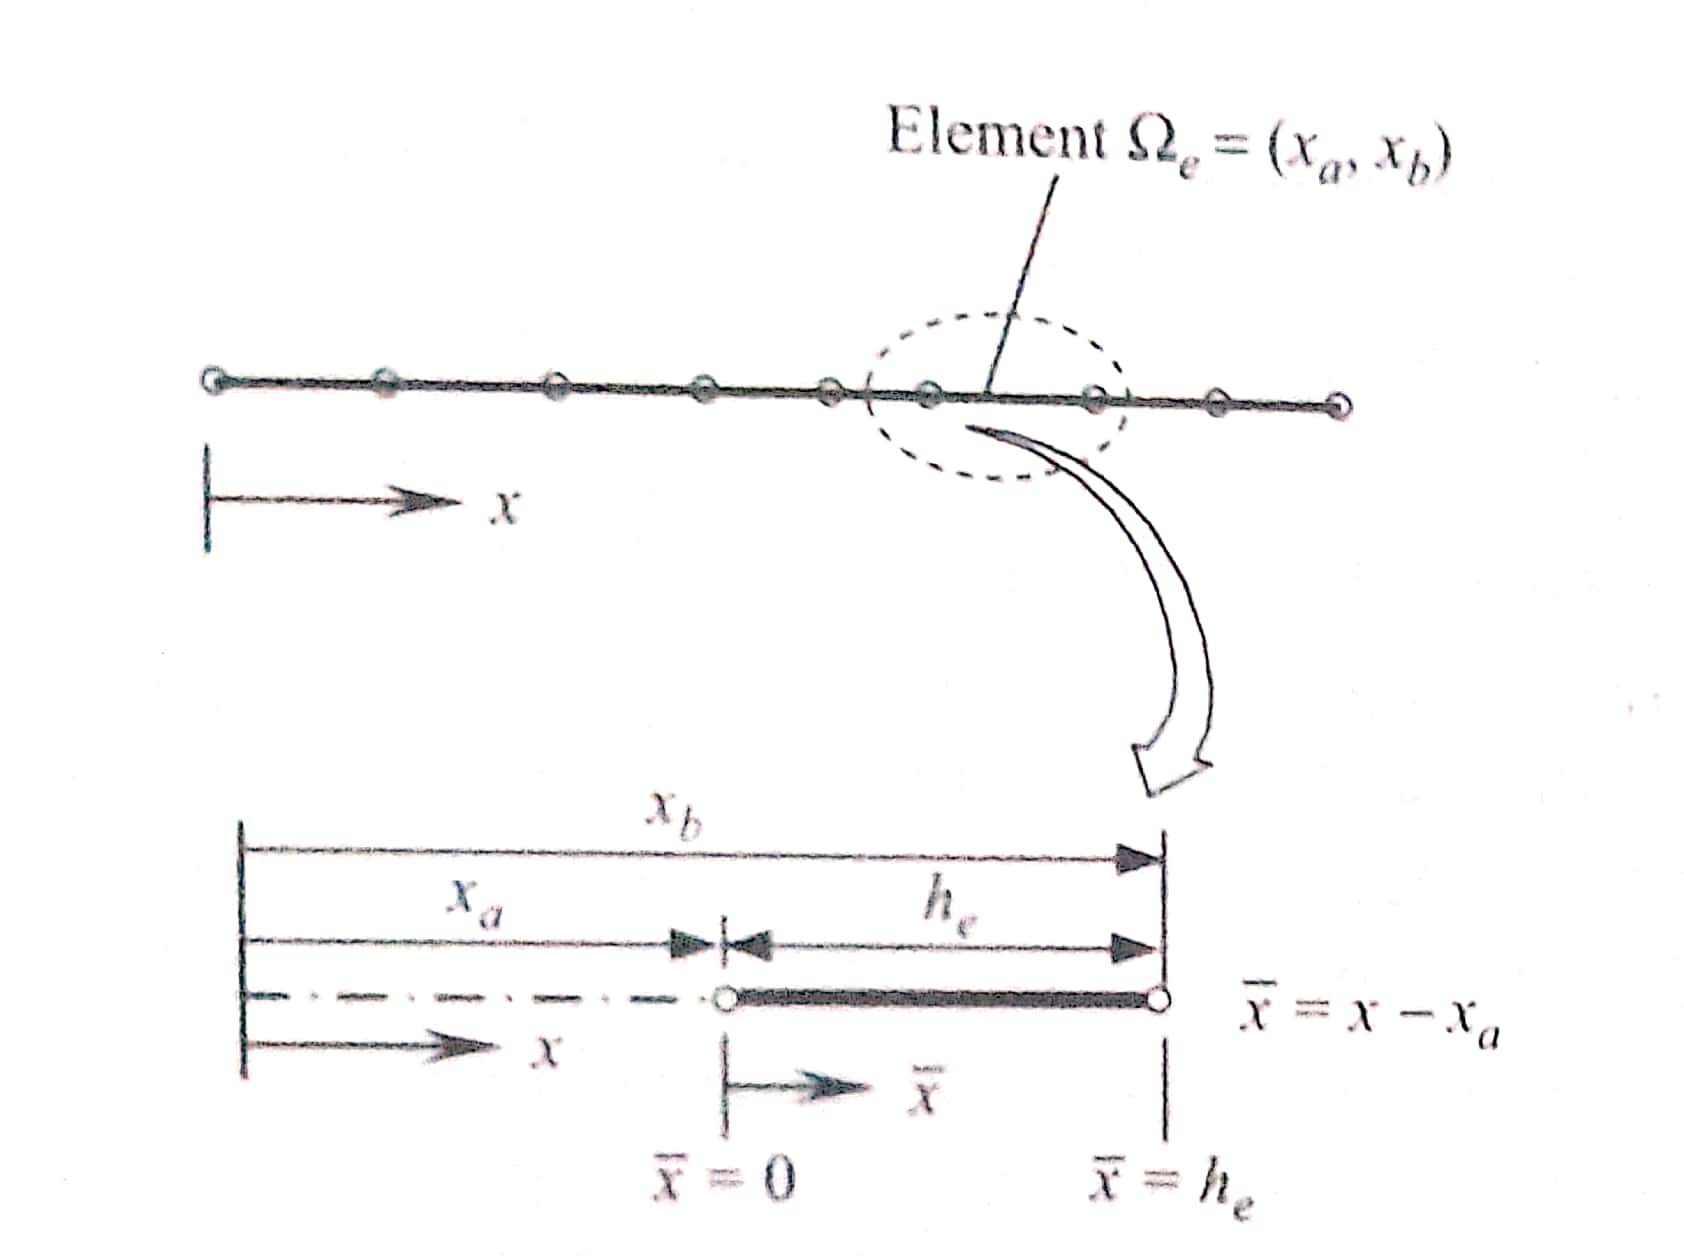
\includegraphics[width=0.9\linewidth , height=0.4\linewidth]{T4}
	\caption{Local Coordinate system for elements}
\end{figure}
where $\bar{x} = x - x_a$

From eqn \ref{gencoeff} we obtain
\begin{eqnarray}
	K_{ij}^e = B(\psi_i^e , \psi_j^e) = \int_{x_a}^{x_b} a_e \frac{d\psi_j^e}{dx} \frac{d\psi_i^e}{dx} dx \\
	F_i^e = l(\psi_i^e) = \int_{x_a}^{x_b} f\psi_i^e dx
\end{eqnarray}

Taking local coordinate $\bar{x}$,
\begin{eqnarray}
	K_{ij}^e =  \int_{0}^{h_e} aE \frac{d\psi_j^e}{d\bar{x}} \frac{d\psi_i^e}{d\bar{x}} d\bar{x} \\
	F_i^e= \int_{0}^{h_e} f\psi_i^e d\bar{x}
\end{eqnarray}

subsituting eqn \ref{locallagrange} , 
\begin{eqnarray}
	K_{11}^e =  \int_{0}^{h_e} a_e \left( - \frac{1}{h_e}\right) \left( - \frac{1}{h_e}\right) d\bar{x} \\
	\implies K_{11}^e = \frac{a_e}{h_e}
\end{eqnarray}

similarly,
\begin{eqnarray}
	 K_{12}^e = K_{21}^e = -\frac{a_e}{h_e}\\
	 K_{22}^e = \frac{a_e}{h_e}
\end{eqnarray}

we can also assume constant $f_e$ to obtain ,
\begin{eqnarray}
	f_{1}^e = 	f_{2}^e = \frac{f_e h_e}{2}
\end{eqnarray}

Hence,
\begin{eqnarray}\label{stiffness}
	[K^e] = \frac{a_e}{h_e}
	\begin{bmatrix}
		1 & -1\\
		-1 & 1
	\end{bmatrix},\quad\quad\quad
	[f^e] = \frac{f_e h_e}{2}
\begin{bmatrix}
	1 \\
	1
\end{bmatrix}
\end{eqnarray}

Summarizing we have obtained the following system,
\begin{eqnarray}\label{system1}
	\frac{a_e}{h_e}
	\begin{bmatrix}
		1 & -1\\
		-1 & 1
	\end{bmatrix}
\begin{bmatrix}
	u_1^e \\
	u_2^e
\end{bmatrix}
 = \frac{f_e h_e}{2}
\begin{bmatrix}
	1 \\
	1
\end{bmatrix} + 
\begin{bmatrix}
	Q_1^e \\
	Q_2^e
\end{bmatrix}
\end{eqnarray}


The above linear system, cannot be solved for each element as it has more variables than there are equations. Thus, we will now combine back our elements to obtain the entire problem domain.

We will be putting additional constraints that $u(x)$ is continuous and source terms are balanced.

Mathematically, If node i of $\Omega_a$ , node j of $\Omega_b$ and  node k of $\Omega_c$ , then 
\begin{eqnarray}
	u_i^a = u_j^b = u_k^c\\
	Q_i^a + Q_j^b + Q_k^c = Q_I
\end{eqnarray}
where , $Q_I$ is externally applied point source

The corresponding matrices of each element must also be added to ensure consistency when external point source are added.
For example,
In the figure below,
    \begin{figure}[h!]
	\centering
	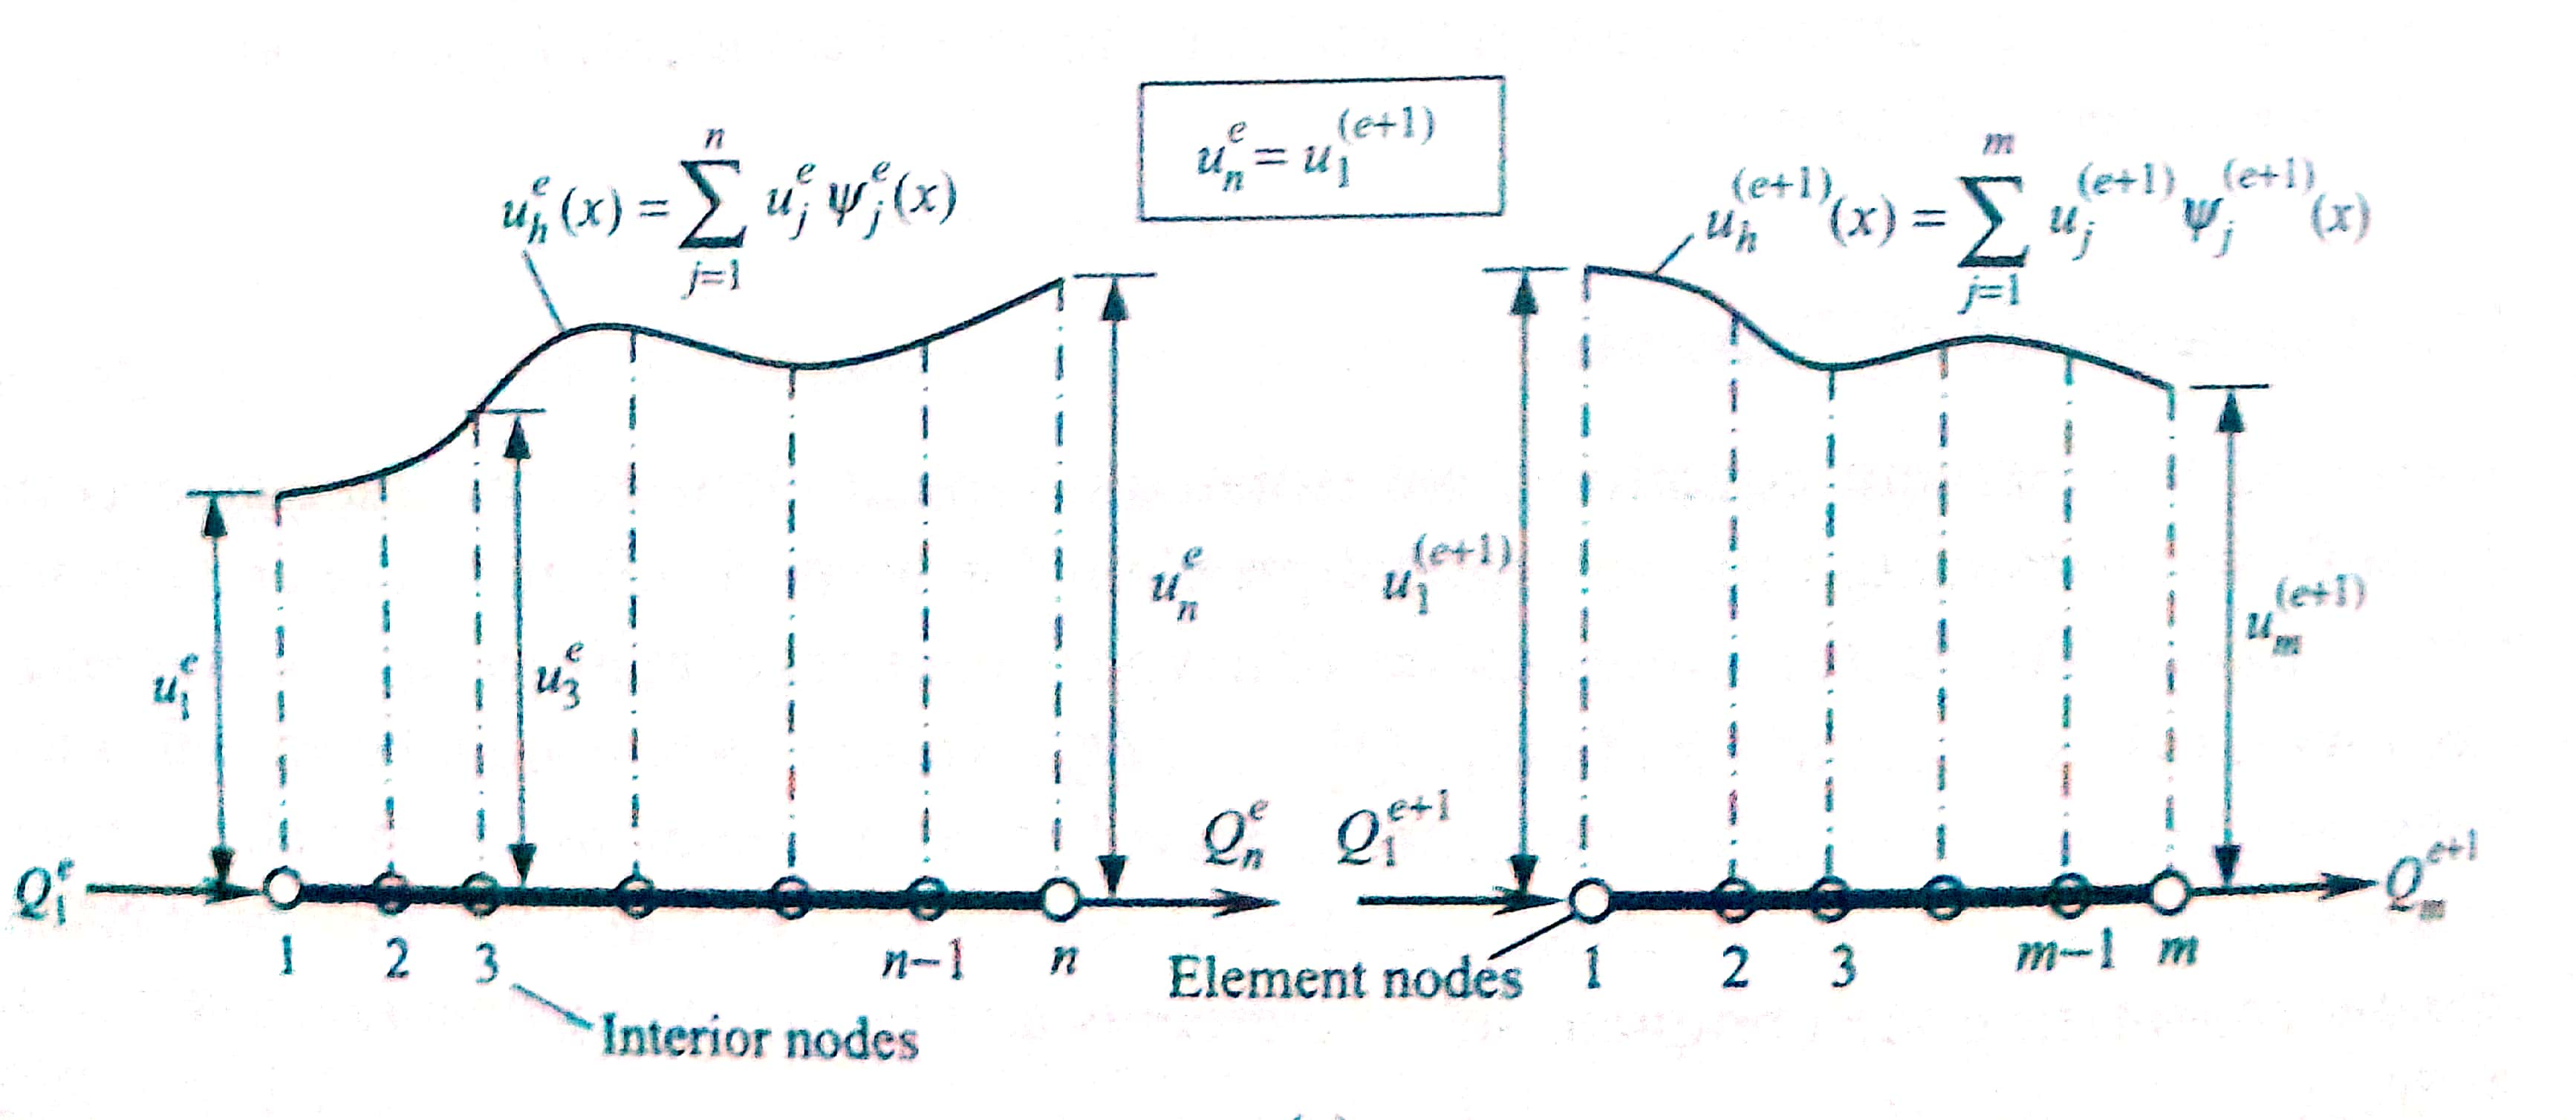
\includegraphics[width=0.9\linewidth , height=0.4\linewidth]{T7}
	\caption{Example of basic Assembly of elements}
\end{figure}
\begin{eqnarray}
	u_1^1 = U_1 , \quad	u_2^1 = u_1^2 =  U_2,  \dots 	u_2^i = u_1^{i+1} =  U_i , \dots u_2^N = U_{N+1}
\end{eqnarray}
    \begin{figure}[h!]
	\centering
	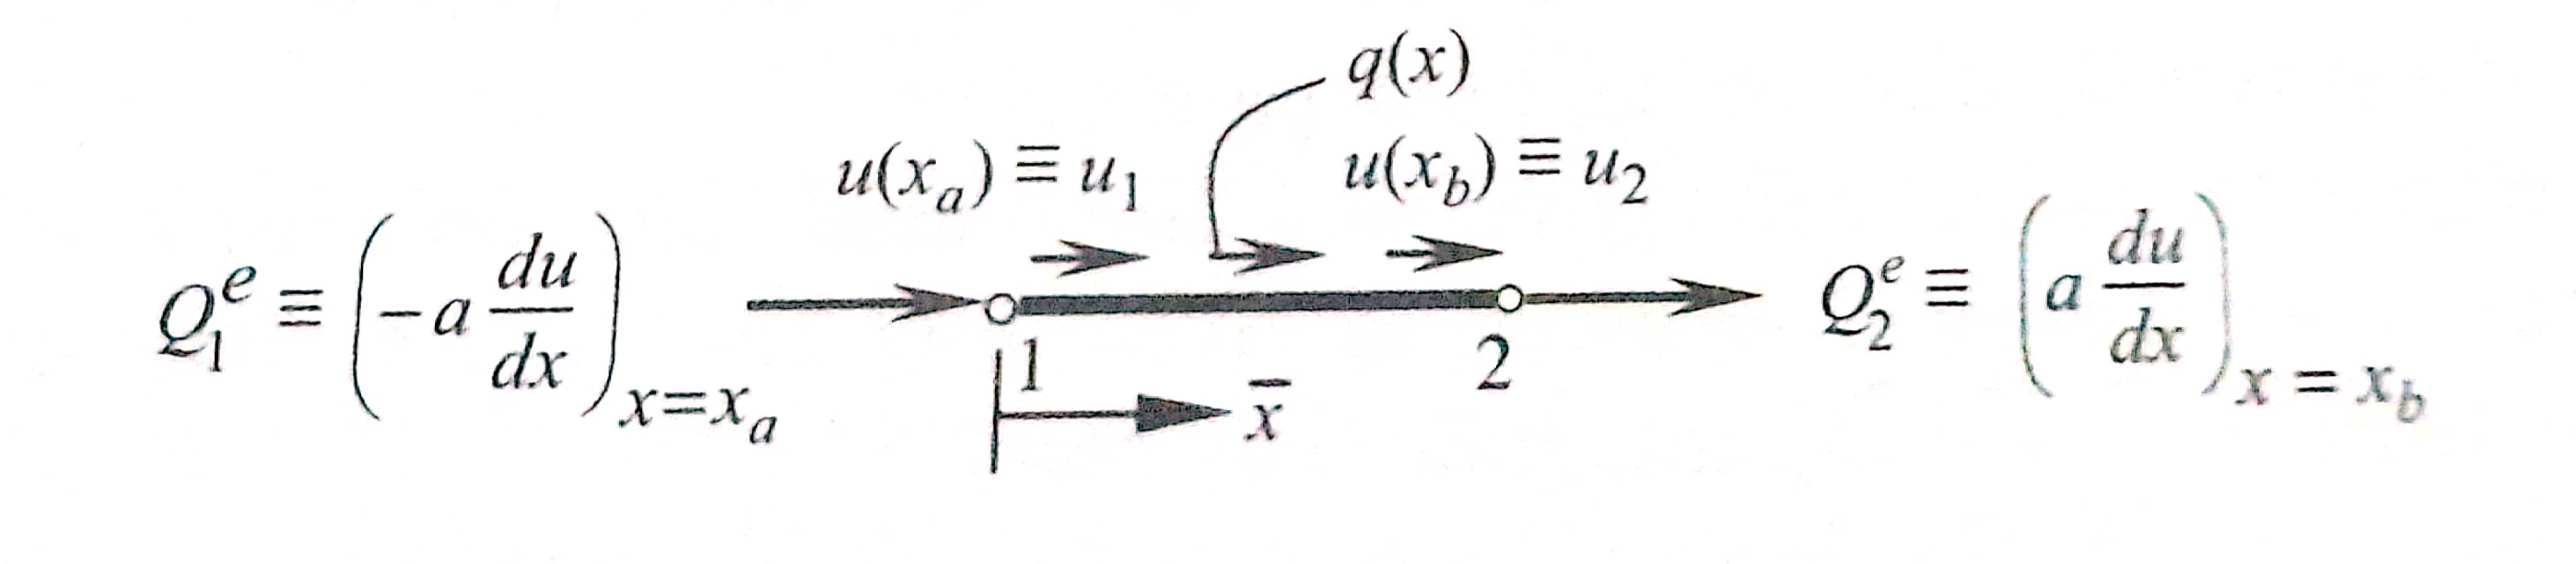
\includegraphics[width=0.9\linewidth , height=0.4\linewidth]{T5}
	\caption{Assembly process for Secondary Variables}
\end{figure}
\begin{eqnarray}
	Q_2^i + Q_1^{i+1} = 0 \quad \text{if no external point source is applied.}\\ \text{otherwise} \quad
	Q_2^i + Q_1^{i+1} = Q_I 
\end{eqnarray}

where $Q_I$ is the magnitude of the external point source applied.

Adding eqn \ref{system1} for sucessive elements, we get


\begin{eqnarray*}
\begin{bmatrix}
		K_{11}^1 & K_{12}^1 & 0 & \dots & 0 & 0 \\
		K_{21}^1 & K_{22}^1 + K_{11}^2 & K_{12}^2 & \dots & 0 & 0 \\
		0 & K_{21}^2 & K_{22}^2 + K_{11}^3 & \dots& 0 & 0 \\
		\vdots & \vdots & \vdots & \vdots & \vdots & \vdots \\
		0 &0 & 0 & \dots & K_{22}^{N-1} + K_{22}^N & K_{12}^N \\
		0 & 0 & 0 & \dots & K_{21}^N & K_{22}^N \\
\end{bmatrix}
\begin{bmatrix}
	U_1 \\
	U_2 \\
	U_3 \\
	\vdots \\
	U_{N-1} \\
	U_N
\end{bmatrix}\\=
\begin{bmatrix}
	f_1^1 \\
	f_2^1 + f_1^2\\
	f_2^2 + f_1^3\\
	\vdots \\
	f_2^{N-1} + f_1^N \\
	f_2^N
\end{bmatrix} +
\begin{bmatrix}
	Q_1^1 \\
	Q_2^1 + Q_1^2\\
	Q_2^2 + Q_1^3\\
	\vdots \\
	Q_2^{N-1} + Q_1^N \\
	Q_2^N
\end{bmatrix} 
\end{eqnarray*}

Now we can impose the boundary conditions on the by providing the values of $U_i$ and $Q_i$ and solve the equation to obtain the solution at the nodal values.
    \begin{figure}[h!]
	\centering
	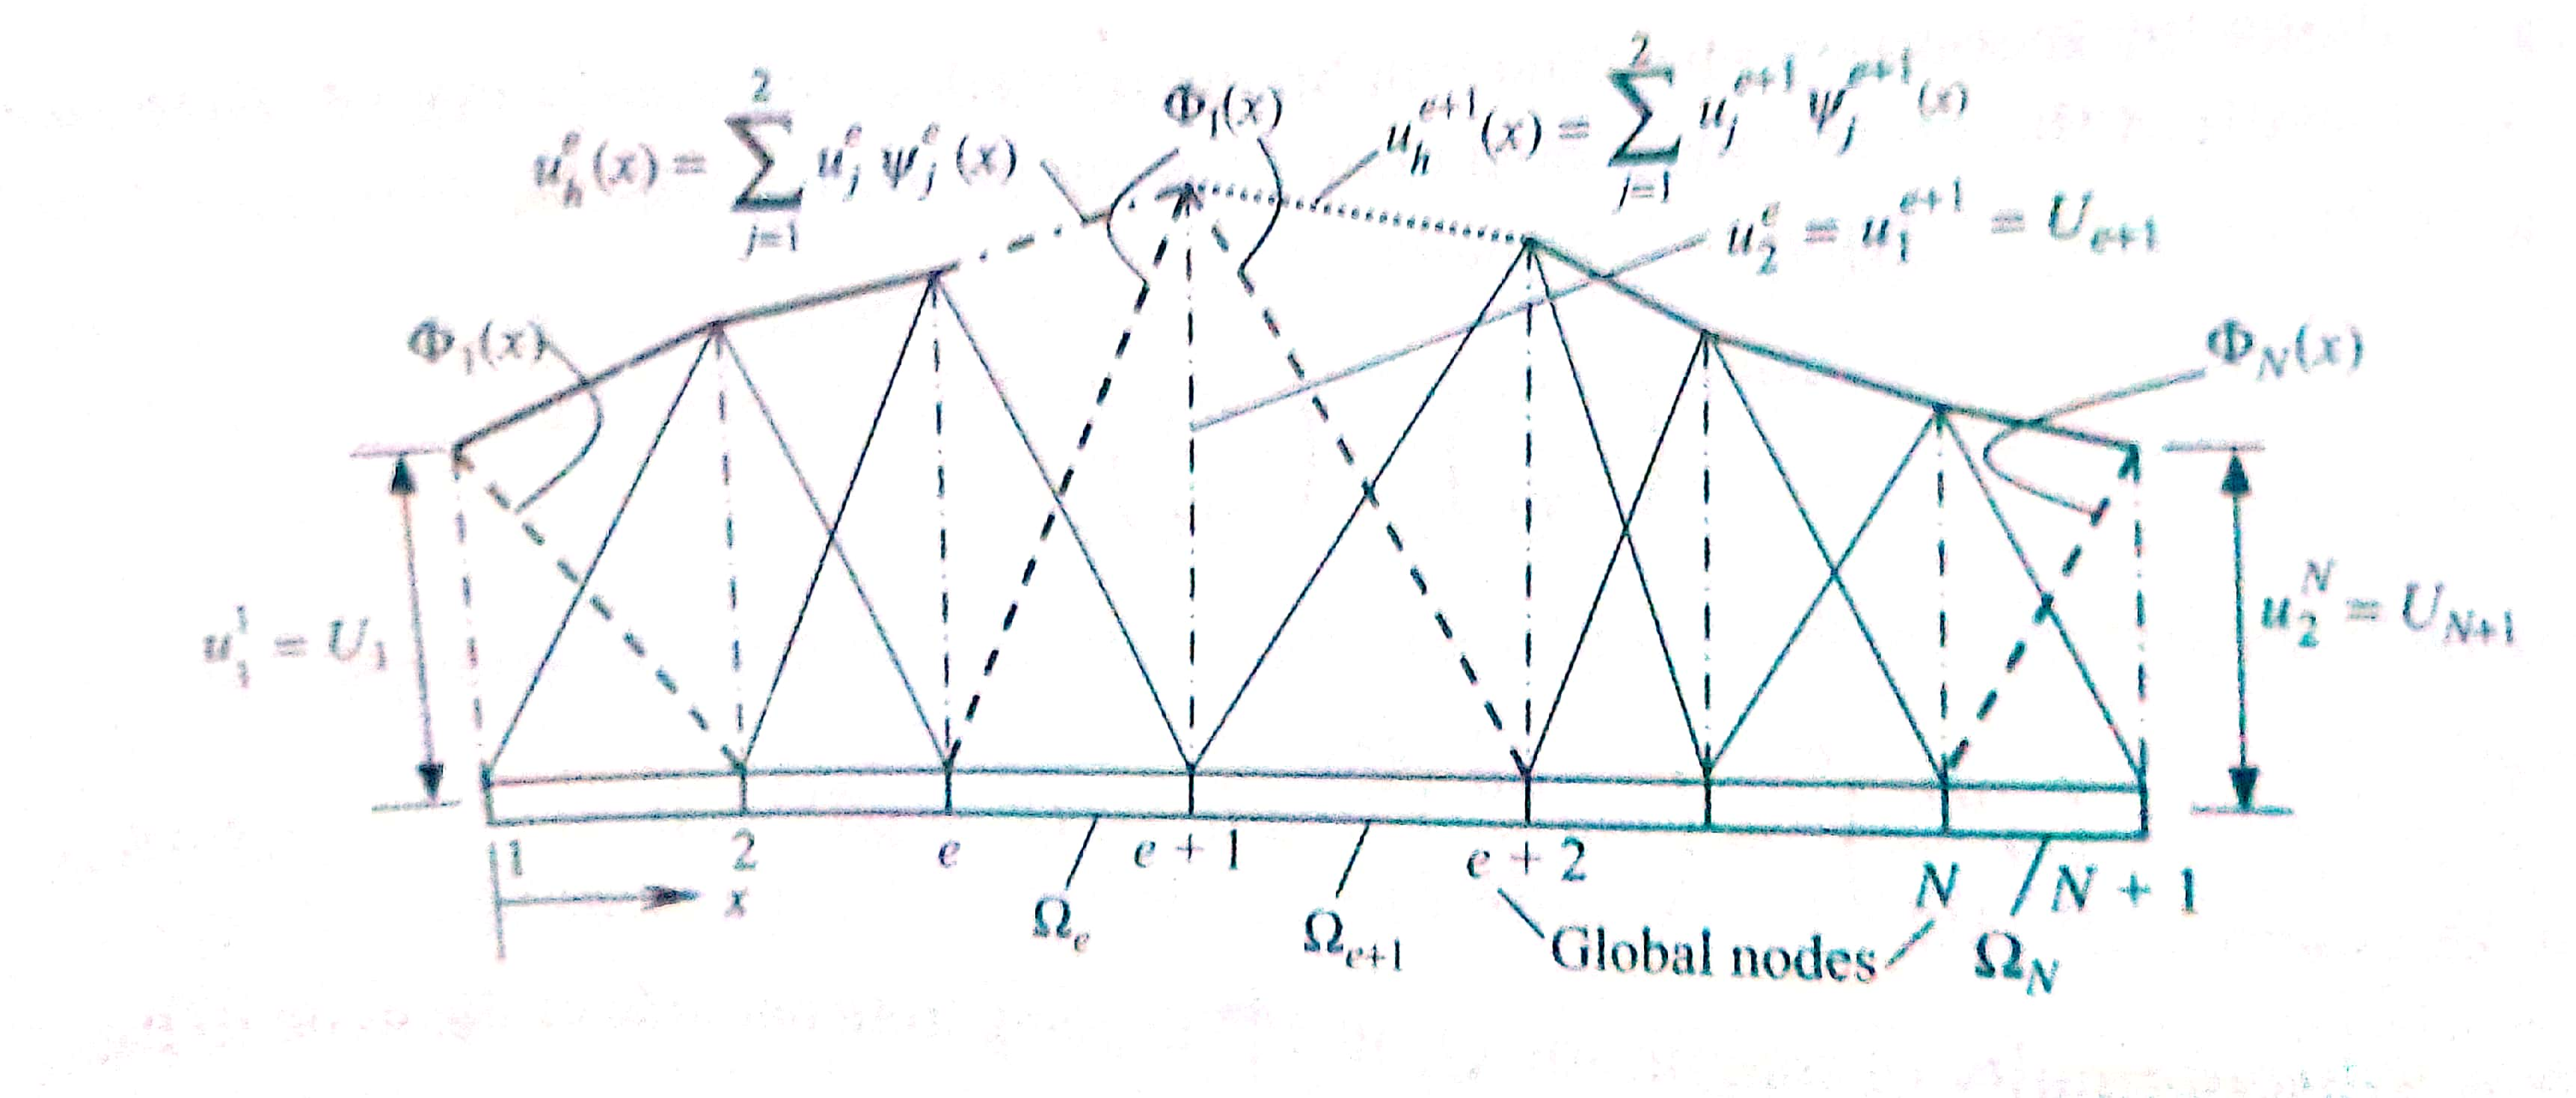
\includegraphics[width=0.9\linewidth , height=0.35\linewidth]{T9}
	\caption{Obtaining Global solution from element solutions}
\end{figure}
The final solution can be written as
\[ u(x) = \begin{cases} 
	u_h^1(x) = \sum_{j=1}^{n} u_j^1 \psi_j^1(x)& x \in \Omega^1 \\
	u_h^2(x) = \sum_{j=1}^{n} u_j^2 \psi_j^2(x)& x \in \Omega^2 \\
	\vdots\\
	u_h^N(x) = \sum_{j=1}^{n} u_j^N \psi_j^N(x)& x \in \Omega^N \\
\end{cases}
\]


In case of Truss, \ref{stiffness} can be written as
\begin{eqnarray}
	[K^e] = \frac{E_e A_e}{h_e}
\begin{bmatrix}
	1 & -1\\
	-1 & 1
\end{bmatrix},\quad\quad\quad
\end{eqnarray}
as $a_e = A_e E_e$ for a bar

We can embed this truss element along x-axis by placing it in 2D plane.
then,
\begin{eqnarray}
	\frac{E_e A_e}{h_e}
	\begin{bmatrix}
		1 & 0 & -1 & 0\\
		0 & 0 & 0 & 0\\
		-1 & 0 & 1 & 0\\
		0 & 0 & 0 & 0
	\end{bmatrix}
	\begin{bmatrix}
		\bar{u_1^e} \\
		\bar{v_2^e} \\
		\bar{u_1^e} \\
		\bar{v_2^e}
	\end{bmatrix}
	= 	\begin{bmatrix}
		\bar{F_1^e} \\
		0 \\
		\bar{F_1^e} \\
		0
	\end{bmatrix}
\end{eqnarray}

This can be expressed as
\begin{eqnarray}	
	[\bar{K^e}]\{\bar{\Delta^e}\} = \{\bar{F^e}\}
\end{eqnarray}

Here we have used the $\bar{x}$  to emphasize that these are local coordinates of the element.
also $\bar{F_1^e} = \bar{f_1^e} + \bar{Q_1^e}$. $\bar{u_1^e}$ and $ \bar{v_2^e} $ denote the displacement along local x and y -axis respectively. 
    \begin{figure}[h!]
	\centering
	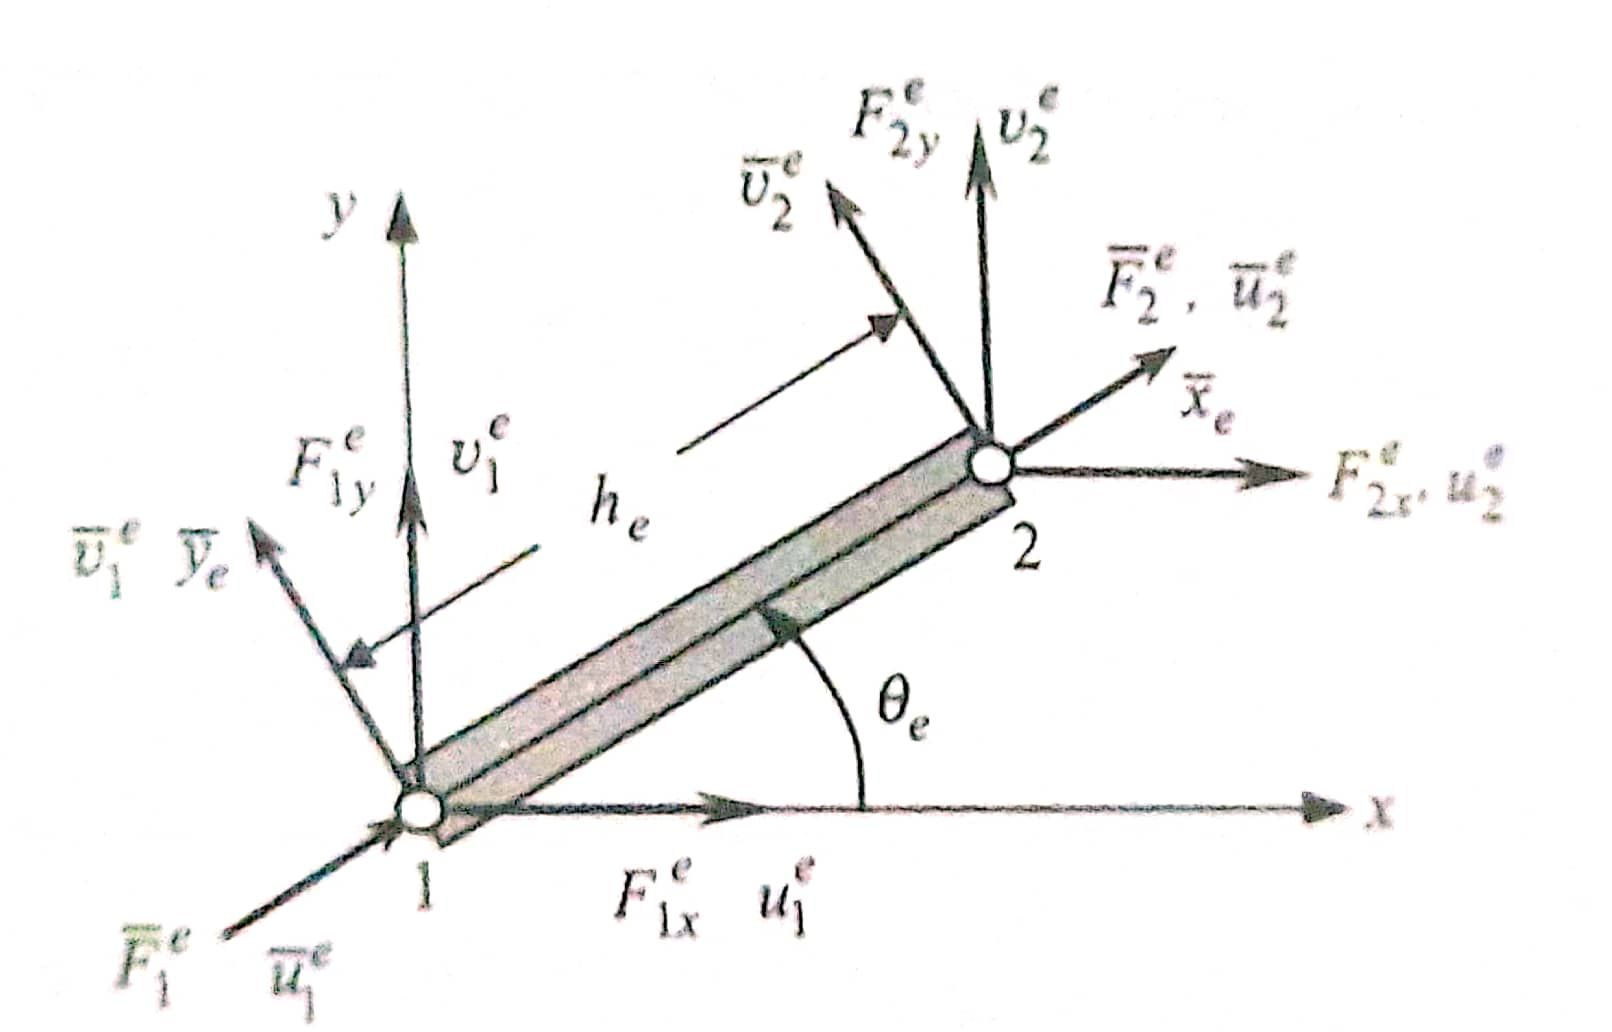
\includegraphics[width=0.8\linewidth , height=0.5\linewidth]{T3}
	\caption{A typical Truss Element}
\end{figure}
Now let us suppose that the element is placed making angle $\theta_e$ with the x-axis. Then The transformation matrix to convert from local to global are,
\begin{eqnarray}
	\begin{bmatrix}
	x \\
	y \\
	\end{bmatrix}
	\begin{bmatrix}
		\cos{\theta_e} & -\sin{\theta_e} \\
		\sin{\theta_e} & \cos{\theta_e} 
	\end{bmatrix}
	\begin{bmatrix}
		\bar{x_e} \\
		\bar{y_e}
	\end{bmatrix}
\end{eqnarray}

Using the above transformation for displacements and forces
\begin{eqnarray}
\begin{bmatrix}
	\bar{u_1^e} \\
	\bar{v_2^e} \\
	\bar{u_1^e} \\
	\bar{v_2^e}
\end{bmatrix} =
\begin{bmatrix}
		\cos{\theta_e} & -\sin{\theta_e} & 0 & 0\\
		\sin{\theta_e} & \cos{\theta_e} & 0 & 0\\
		0 &  0 &\cos{\theta_e} & -\sin{\theta_e} \\
		0& 0& \sin{\theta_e} & \cos{\theta_e}  
\end{bmatrix}
\begin{bmatrix}
{u_1^e} \\
{v_2^e} \\
{u_1^e} \\
{v_2^e}
\end{bmatrix}
\end{eqnarray}

\begin{eqnarray}	
\{\bar{\Delta^e}\} = [T^e]  \{\Delta^e\}
\end{eqnarray}
\begin{eqnarray}	
\{\bar{F^e}\} = [T^e]  \{F^e\}
\end{eqnarray}

\begin{eqnarray}	
	[\bar{K^e}][T^e]  \{\Delta^e\} = [T^e]  \{F^e\}\\
	\implies [T^e]^T [\bar{K^e}] [T^e] {\bar{\Delta^e}} =  [T^e]^T \{\bar{F^e}\}\\
\end{eqnarray}

let 
\begin{eqnarray}
	\{ F^e \}=[T^e]^T \{ \bar{F^e} \}
\end{eqnarray}
\begin{eqnarray}
	[K^e] =  [T^e]^T [\bar{K^e}] [T^e]
\end{eqnarray}

So finally we can write,
\begin{eqnarray}	
	[{K^e}]\{{\Delta^e}\} = \{{F^e}\}
\end{eqnarray}

where,
\begin{eqnarray}
[K^e] = \frac{E_e A_e}{h_e}
	\begin{bmatrix}
		\cos^2{\theta_e} & \frac{1}{2}\sin{2\theta_e} & -\cos^2{\theta_e} & -\frac{1}{2}\sin{2\theta_e}\\
		\frac{1}{2}\sin{2\theta_e} & \sin^2{\theta_e} & -\frac{1}{2}\sin{2\theta_e} & -\sin^2{\theta_e}\\
			-\cos^2{\theta_e} & -\frac{1}{2}\sin{2\theta_e} & \cos^2{\theta_e} & \frac{1}{2}\sin{2\theta_e}\\
		-\frac{1}{2}\sin{2\theta_e} & -\sin^2{\theta_e} & \frac{1}{2}\sin{2\theta_e} & \sin^2{\theta_e}\\
	\end{bmatrix}
\end{eqnarray}
\pagebreak

Further process is identical to the assembly and solving linear equations as we explained above.
\section{\bf Python Implementation}

\subsection{Input/Output}
To feed the data to our program, we came up with the idea of using csv files so as to make the program available for general problems and for a easy to use input interface.\\


\begin{table}[h!]
	\centering
	\begin{tabular}{|l|l|l|l|l|l|l|}
		\hline
		Node & x\_pos & y\_pos & x\_dis & y\_dis & x\_force & y\_force \\
		\hline
		1    & 0      & 0      & 0      & 0      & 0        & 0        \\
		2    & 2      & 0      & 0      & 0      & 0        & 0        \\
		3    & 4      & 0      & 0      & 0      & 0        & 0        \\
		4    & 6      & 0      & 0      & 0      & 0        & 0        \\
		5    & 8      & 0      & 0      & 0      & 0        & 0        \\
		6    & 8      & 2.918  & nan    & nan    & 0.2      & -0.1     \\
		7    & 6      & 2.1838 & nan    & nan    & 0        & -0.1     \\
		8    & 4      & 1.4559 & nan    & nan    & 0        & -0.1     \\
		9    & 2      & 0.7279 & nan    & nan    & 0        & -0.1  	\\
		\hline  
	\end{tabular}
		\caption{Example of a CSV file used to input node data}
	\label{node_csv_table}
\end{table}

Table \ref{node_csv_table}shows the input format of nodes where each row represents a node and its various attributes in the specified columns. Going from left to right we get node number, position , displacements and external force applied along the local x and y-axis.\\

The values that are unknown and thus to be computed will be denoted by nan and any geometry and boundary conditions can be specified in this table.

\begin{table}[h!]
	\centering
	\begin{tabular}{|l|l|l|l|l|l|l|}
		\hline
		Element & Length & CS-Area & Young's Modulus & Global Angle & Start node & End node \\
		\hline
		1               & 2      & 1                    & 1              & pi*0         & 1             & 2           \\
		2               & 2      & 1                    & 1              & pi*0         & 2             & 3           \\
		3               & 2      & 1                    & 1              & pi*0         & 3             & 4           \\
		4               & 2      & 1                    & 1              & pi*0         & 4             & 5           \\
		5               & 2.9118 & 1                    & 1              & pi*0.5       & 5             & 6           \\
		6               & 2.1284 & 1                    & 1              & pi*0.11111   & 7             & 6           \\
     	\hline
	\end{tabular}
	\caption{Example of a CSV file used to input element data}
	\label{element_csv_table}
\end{table}


Table \ref{element_csv_table} shows the input format of the elements where each row represents an element and its attributes: element number, length , cross-section area , young's modulus , angle with the global x-axis and the nodes that it connects. We can use this table to supply material properties and specify the problem geometry.

The output is similarly given as a CSV file.

\subsection{Element and Node classes}
The input from csv files are then used to define the objects of two classes namely node and ele. These class have all the attributes needed and methods to be able to easily manipulate and visualize them.

Formation of global stiffness matrix was a challenge and reducing the code to faster execution and simplicity was even bigger of a task. Finally the method applied is as follows.


\begin{lstlisting}[language=Python , basicstyle=\linespread{0.75}\listingsfont]
	def globalstiff(eles , num_nodes):
		#dimension of global matrix
		dim = 2 * num_nodes
		#generate and store the element-wise stiffness matrices
		SMs = [e.stiff() for e in eles]
	
		GK = np.zeros((dim,dim))
		
		for e in eles:
			i = 2 * e.node_a.num -2
			j = 2 * e.node_a.num -1
			k = 2 * e.node_b.num -2
			l = 2 * e.node_b.num -1
			e_stiff = e.stiff()
	
			index = [i,j,k,l]
			index2d = [(a,b) for a in index for b in index]
			d = {i:0, j:1, k:2, l:3}
			
			for p,q in index2d:
			    GK[p][q] = GK[p][q] + e_stiff[d[p]][d[q]]
		
		return GK
\end{lstlisting}

The list of elements is iterated throughout for accessing each element. Then with the logic of how the values in local stiffness matrix is appended to the global matrix, we came up with an efficient algorithm that fits well to our purpose as well as works on all such general problems with slightest of tweaks.

After generating global stiffness matrix we now had 3 variables: the stiffness matrix , the displacement and the force vector. For simplifying the calculations and faster computation, for $n^{th}$ element which was specified in the displacement vector, we reduced the global matrix by removing corresponding $n^{th}$ row and columns by changing the secondary variable accordingly.  After reduction simple linear algebra has been applied to find out the unknown/missing values of displacement of each node. 

\begin{lstlisting}[language=Python , basicstyle=\linespread{0.75}\listingsfont]
#check for undetermined values in dis and create linear eqns

GK_dis =  copy.deepcopy(GK)
f_dis =  copy.deepcopy(f)

#get a list of rows to remove
del_row = []

index_list = list(range(0,2*len(nodes)))
for i in range(0,2*len(nodes)):
    if not np.isnan(dis_list[i]):
        del_row.append(i)
        index_list.remove(i)

#remove the rows that have displacement given
GK_dis = np.delete(GK_dis,del_row,0)
f_dis = np.delete(f_dis,del_row,0)

#before deleting the columns we subratct these from force vector
for i in del_row:
        f_dis = f_dis - dis_list[i] * GK_dis[:,i]

#delete the columns that are due to the displacements that are determined
GK_dis = np.delete(GK_dis,del_row,1)
\end{lstlisting}


\subsection{Visualization}
For the last and final part of visualizing our problem and the visualizing the solution so as to make each bit of data understandable we used the Turtle module of Python. Initially we draw our problem provided the position of the nodes and elements connecting them.

\begin{lstlisting}[language=Python , basicstyle=\linespread{0.75}\listingsfont]
	for ele in self.ele_list:
	t.goto(ele.node_a.pos_x, ele.node_a.pos_y)
	t.pendown()
	t.goto(ele.node_b.pos_x, ele.node_b.pos_y)
	t.penup()
	
	for node in self.node_list:
	t.penup()
	t.goto(node.pos_x, node.pos_y)
	t.pendown()
	t.dot(15, "red")
	
	t.penup()
	t.goto((ele.node_a.pos_x + ele.node_a.dis_x), (ele.node_a.pos_y + ele.node_a.dis_y))
	t.pendown()

	# after solving
	t.pencolor("green")
	for ele in self.ele_list:
	t.goto((ele.node_a.pos_x + ele.node_a.dis_x), (ele.node_a.pos_y + ele.node_a.dis_y))
	t.pendown()
	t.goto((ele.node_b.pos_x + ele.node_b.dis_x), (ele.node_b.pos_y + ele.node_b.dis_y))
	t.penup()
	
	t.speed(0)
	for node in self.node_list:
	t.penup()
	t.goto((node.pos_x + node.dis_x), (node.pos_y + node.dis_y))
	t.pendown()
	t.dot(15, "yellow")

\end{lstlisting}

 Then using the displacement data of each node that we get after the computation, the same algorithm is applied to draw the final result/ shape of the truss. This time the position of node is the sum of its original position and its displacement in x and y-axis. Different tools have been used to make the visualized problem and result understandable.

